\section{Laplace distribution/ Double Exponential Distribution ( $ {\displaystyle \text {Laplace} (\mu ,b)} $ )}


\begin{table}[H]
    \hfill
    \begin{minipage}{0.45\linewidth}
        \begin{figure}[H]
            \centering
            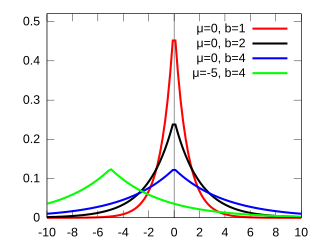
\includegraphics[
                width=\linewidth,
                height=5cm,
                keepaspectratio,
            ]{images/distributions/Laplace_pdf_mod.svg.png}
            \caption{Double Exponential/ Laplace Distribution: PDF \cite{wiki/Laplace_distribution}}
        \end{figure}
    \end{minipage}
    \hfill
    \begin{minipage}{0.45\linewidth}
        \begin{figure}[H]
            \centering
            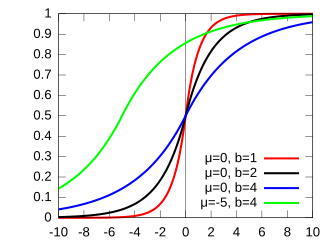
\includegraphics[
                width=\linewidth,
                height=5cm,
                keepaspectratio,
            ]{images/distributions/Laplace_cdf_mod.svg.png}
            \caption{Double Exponential/ Laplace Distribution: CDF \cite{wiki/Laplace_distribution}}
        \end{figure}
    \end{minipage}
    \hfill
\end{table}



\subsection{PDF}

\begin{enumerate}
    \item The double exponential is symmetric, like the normal PDF
    \hfill \cite{statistics/book/Statistics-for-Data-Scientists/Maurits-Kaptein}

    \item The double exponential PDF can easily be determined using the exponential PDF. 
    The double exponential PDF, for any value $x \in \mathbb{R}$, is defined by $0.5 f_\lambda (\dabs{x})$, with $\dabs{\cdot}$ the absolute function.
    \hfill \cite{statistics/book/Statistics-for-Data-Scientists/Maurits-Kaptein}
    \\
    Note: $\mu = 0, b=\dfrac{1}{\lambda}$
    \hfill \cite{common/online/chatgpt}
\end{enumerate}




\subsection{Summary}

\begin{enumerate}
    \item \textbf{Parameters}:
    \hfill \cite{wiki/Laplace_distribution}
    \begin{enumerate}
        \item ${\displaystyle \mu }$ location (real)
        \hfill \cite{wiki/Laplace_distribution}
        
        \item ${\displaystyle b>0}$ scale (real)
        \hfill \cite{wiki/Laplace_distribution}
    \end{enumerate}

    \item \textbf{Support}: $ {\displaystyle \mathbb {R} }$
    \hfill \cite{wiki/Laplace_distribution, statistics/book/Statistics-for-Data-Scientists/Maurits-Kaptein}

    \item \textbf{PDF}:
    $ {\displaystyle {\dfrac {1}{2b}}\exp \left(-{\dfrac {|x-\mu |}{b}}\right)}$
    \hfill \cite{wiki/Laplace_distribution, statistics/book/Statistics-for-Data-Scientists/Maurits-Kaptein}

    \item \textbf{CDF}: $ {\displaystyle {\begin{cases}{\dfrac {1}{2}}\exp \left({\dfrac {x-\mu }{b}}\right)&{\text{if }}x\leq \mu \\[8pt]1-{\dfrac {1}{2}}\exp \left(-{\dfrac {x-\mu }{b}}\right)&{\text{if }}x\geq \mu \end{cases}}}$
    \hfill \cite{wiki/Laplace_distribution}

    \item \textbf{Quantile}: $ {\displaystyle {\begin{cases}\mu +b\ln \left(2F\right)&{\text{if }}F\leq {\dfrac {1}{2}}\\[8pt]\mu -b\ln \left(2-2F\right)&{\text{if }}F\geq {\dfrac {1}{2}}\end{cases}}}$
    \hfill \cite{wiki/Laplace_distribution}

    \item \textbf{Mean}: $ {\displaystyle \mu }$
    \hfill \cite{wiki/Laplace_distribution}

    \item \textbf{Median}: $ {\displaystyle \mu }$
    \hfill \cite{wiki/Laplace_distribution}

    \item \textbf{Mode}: $ {\displaystyle \mu }$
    \hfill \cite{wiki/Laplace_distribution}

    \item \textbf{Variance}: $ {\displaystyle 2b^{2}}$
    \hfill \cite{wiki/Laplace_distribution}

    \item \textbf{Skewness}: $ {\displaystyle 0}$
    \hfill \cite{wiki/Laplace_distribution}

    \item \textbf{Excess kurtosis}: $  {\displaystyle 3} $
    \hfill \cite{wiki/Laplace_distribution}

    \item \textbf{Entropy}: $  {\displaystyle \log(2be)} $
    \hfill \cite{wiki/Laplace_distribution}

    % \item \textbf{Fisher information}: $ $
    % \hfill \cite{wiki/Laplace_distribution}

    \item \textbf{Expected shortfall}:
    $ {\displaystyle {\begin{cases}\mu +b\left({\dfrac {p}{1-p}}\right)(1-\ln(2p))&,p<0.5\\\mu +b\left(1-\ln \left(2(1-p)\right)\right)&,p\geq 0.5\end{cases}}}$
    \hfill \cite{wiki/Laplace_distribution}

    \item \textbf{Moment-generating function (MGF)}: 
    $ {\displaystyle {\dfrac {\exp(\mu t)}{1-b^{2}t^{2}}}{\text{ for }}|t|<1/b}$
    \hfill \cite{wiki/Laplace_distribution}

    \item \textbf{Characteristic function (CF)}:
    $ {\displaystyle {\dfrac {\exp(\mu it)}{1+b^{2}t^{2}}}}$
    \hfill \cite{wiki/Laplace_distribution}

    \item \textbf{Kullback–Leibler divergence}:
    $ $
    \hfill \cite{wiki/Laplace_distribution}

    \item \textbf{Median absolute deviation (MAD)}:
    $ {\displaystyle b\ln 2}$
    \hfill \cite{wiki/Laplace_distribution}
\end{enumerate}











